\documentclass[a4paper]{report}
\usepackage[utf8]{inputenc}
\usepackage[english]{babel}
\usepackage{amsmath}
\usepackage{amssymb}
\usepackage{amsthm}
\usepackage{graphicx}
\usepackage{hyperref}
\usepackage[english]{babel}
\usepackage[autostyle]{csquotes}
\usepackage{float}
\usepackage[font={small,it}]{caption}
\usepackage[top=1in, bottom=1.25in, left=1in, right=1in]{geometry}
\theoremstyle{definition}
\newtheorem{definition}{Definition}[section]
\theoremstyle{remark}
\newtheorem*{remark}{Remark}
\newtheorem*{theorem}{Theorem}

\begin{document}

	%%% Title Page %%%
	\begin{titlepage}
		\title{A quick Look through the mathematical prerqusites for General Theory of Relativity}
		\author{Biplab Mahato\\K Philip Thomas}
		\date{}
		\maketitle
	\end{titlepage}

	%%% Table of Content %%%
	\tableofcontents

	\section{Introduction}
		The general theory of relativity is a theory, which if one wants to see and understand in its full glory, requires one to have a lot of mathematical prerequisites in the fields of calculus, analysis and differential geometry. In this report, we have tried to present a small section of formal mathematical constructions which we learnt over the summer, to understand the Einstein equations. We have defined mathematical objects and tried to give an intuition about the object whenever possible. Few proofs are given, and a few of the proofs are sketched. The report is more of a mathematical nature and the physics part is not given much elaboration. A basic knowledge of multivariable calculus, topology and linear algebra is assumed. All the sections until the last  two are purely of mathematical nature.
	\section{Manifolds}
		Roughly speaking, a manifold is a topological space that \enquote{locally} looks like $\mathbb{R}^n$ for some fixed n, where n is called the dimension of the manifold. One could say that the space is locally \enquote{flat}. From experience, we know that a sphere should intuitively be a manifold of dimension 2. This notion is formalized as follows:
		\begin{definition} 
			A topological space $M$ is called a $d$-dimensional manifold if $\forall  p \in M$, there exist a bijective map $x$ from some open set $U\subset M$ containing $p$ to open set $V \subset \mathbb{R}^d $ such that $ x$ and $x^{-1}$ are continuous(Such a map $x$ is called a \emph{homeomorphism} between $U$ and $V$).
		\end{definition}
		We call such pairs $(U,x)$ as \emph{charts} and $x$ as a \emph{chart map}. We see that by using $x$ you can see the space locally in $\mathbb{R}^d$, i.e acts as a local coordinate system on the manifold. An immediate consequence is that you have a collection of these charts, say $\mathcal{A}$ so that for any point you have some chart which maps a neighbourhood of it to $\mathbb{R}^d$. 
		We say that two charts $(U,x)$ and $(V,y)$ to be $C^k$-compatible if $(x\circ y^{-1})$ and $(y\circ x^{-1})$ (These functions are called \emph{chart transition maps}) are $C^k$ functions on their respective domains, where a function being $C^k$ means it is differentiable k times.
		Note that $\mathcal{A}$ as above consists of compatible $C^0$ charts.This motivates the definition for a smooth manifold, meaning the ‘local maps’ are smooth.
		\begin{definition}
			An smooth atlas $\mathcal{A}$ on $M$ is a collection of charts $(U_{\alpha},x_{\alpha})$(not necessarily countable) such that the chart transition maps are smooth and $\bigcup\limits_{\alpha}U_{\alpha} = M$\end{definition}
		\begin{definition}
			A d-dimensional manifold M along with a smooth atlas is called a smooth manifold of dimension d.
		\end{definition}
		One usually adds the further condition that an atlas be maximal (i.e contains all compatible charts) so that two equivalent spaces (upto a diffeomorphism) equipped with different atlases are not counted as different manifolds. Also every atlas is contained in a unique maximal atlas.
		Example: Of course, $\mathbb{R}^n$ is a smooth manifold of dimension n.
			%S2 := \dots\dots, the unit sphere in R3 centered at origin, is made into a smooth manifold using the stereographic projections :\dots\dots\dots 
			\\
		This imposition of smoothness to the chart maps help us generalize differentiability of functions between manifolds in the following way:
		\begin{definition}
			A function $f:M\to N$ is smooth at $p \in M$ if there exist chart $(U,x)$ and $(V,y)$ such that $p\in U$, $f(p) \in V$  and $(y\circ f\circ x^{-1}): x(U) \to y(V)$ is smooth. \end{definition}
		It is easy to see that if for one chart the above condition holds, then compatibility of charts imply that it holds for all charts. Hence it is a well-defined notion. We say $f$ is smooth if it is smooth at every point in $M$.
	\section{Multilinear algebra}
		We shall deal with vector spaces over the field $\mathbb{R}$.
		Let $V$ be a vector space.
		\begin{definition}
			The dual space of $V$, $V^*$ := set of all linear maps from $V$ to $\mathbb{R}$ along with '+','$\cdot$' defined as below
			\begin{eqnarray*}
				(F+G)(v) &:=&F(v) + G(v) \\ (c.F)(v) &:=&  cF(v) 
			\end{eqnarray*}
			where $c \in \mathbb{R}$, $F,G \in V^*$, so that $(V^*,+,.)$ is a vector space.
		\end{definition}
		For finite dimensional vector space $V$, let $(e_i)$ be a bases, then we have $e^i: e^i(e_j) = \delta^i_j$  to form a basis of V*. Elements of $V^*$ are called co-vectors.
		\begin{definition}
			A $(p,q)$-tensor $T$ is a multilinear map $T:V^{*p} \times V^q \to \mathbb{R}$ , i.e. $T$ is linear in each of its arguments.
		\end{definition}
		For example:\\
		Every covector is a (0,1) tensor. \\
		If $T$ is a $(1,1)$-tensor, it takes in a dual vector and a  vector to output a scalar. Given an endomorphism G of V (i.e. a linear transformation from V to V), one has the $(1,1)$ tensor $T$ such that $T(w^*,v) = w^*(G(v))$. \\
		One important example is that of the inner product, which is a symmetric , non-degenerate $(0,2)$ tensor, usually depicted by $g$(where non-degeneracy means $g(v_1,v_2) = 0$ for any $v_2 \implies v_1=0$). The Minkowskian metric $\eta$ is an important example from special relativity. \\
		The set $T^{ p}_qV$ of $(p,q)$-tensors can be given a vector space structure by pointwise addition and scaling at each evaluation. It is called the $(p,q)$-tensor space over $V$.
		\begin{definition}
			Given $(p,q)$ , $(r,s)$ tensors $T$ and $Q$ respectively, one can define a $(p+r,q+s)$ tensor $T\otimes Q$:
		\begin{equation*}
		T\otimes Q(w_1,..,w_p,w_{p+1},..w_{p+r},v_1,..,v_{q+s})=T(w_1,..,w_p,v_1,..v_q).Q(w_{p+1},..w_{p+r},v_{q+1},..,v_{q+s})\end{equation*}\end{definition}
		Thus tensor product lets us construct new tensors from other tensors. One other way of getting new tensor is by contracting a tensor. We will come to this later.
		Suppose $V$ has basis ${e_i}$, $i\leq n$ .Then we have a basis for the $(p,q)$ tensor space over V , given by $e_{j_1}\otimes \dots \otimes e_{j_p}\otimes e^{i_1}\otimes \dots\otimes e^{i_q}$ where $j_1,\dots,j_p,i_1,\dots,i_q\leq n$, where the component of the $(p,q)$ tensor T is given by $T(e^{j_1},\dots,e_{i_q})$ with respect to the basis element $e_{j_1}\otimes\dots\otimes e_{j_p}\otimes e^{i_1}\otimes \dots\otimes e^{i_q}$.
		Denoted by 
		\begin{eqnarray*}
			T&=& T(e^{j_1},\dots,e_{i_q})e_{j_1}\otimes\dots\otimes e_{j_p}\otimes e^{i_1}\otimes \dots\otimes e^{i_q} \\
			&=& T^{\hspace{2pt}j_1...j_p}_{i_1...i_q}e_{j_1}\otimes\dots\otimes e_{j_p}\otimes e^{i_1}\otimes \dots\otimes e^{i_q}
		\end{eqnarray*}
		\begin{remark}
			We shall be following the Einstein Summation convention so that whenever an index is there as a subscript and superscript in the same term, we mean the sum over the index.
		\end{remark}
		Given a $(p,q)$-tensor $T$, $p$ and $q > 0$, we have a $(p-1,q-1)$-tensor $Q$  by plugging in a basis element $e_i$ of $V$ and its corresponding dual $e^i$ of V* in T and taking the sum, i.e,
		$Q=\sum_{i} T(.,\dots,e^i,\dots,e_i,\dots)$
		It can be checked easily that Q defined in this way is again a multilinear map and hence a valid tensor, moreover the components of this tensor are:
		\begin{equation*}
			Q^{\hspace{2pt}j_1...j_{p-1}}_{\hspace{0pt}i_1...i_{q-1}} = \sum_{j_k}T^{\hspace{2pt}j_1.,j_k,..j_p}_{\hspace{2pt}i_1.,j_k,..i_q}
		\end{equation*}
		\textbf{Change of basis:}
		First let us consider how vectors and co-vectors behave under basis transformations.
		Let $\mathcal{B} = (e_i)$ and $\mathcal{B'}= (e’_j)$ be two bases of $V$. Let $e_i = A_i^j e’_j$, Then if vector $v = v^j e_j = v'^j e’_j$ (note that upon change of basis vector itself does not change but its components do change as follows),
		Then 
		\begin{eqnarray*}
			v&=&v^i A_i^j e’_j = v'^j e’_j\\ &\implies & v^i A_i^j = v'^j  \\
			&& v^i = v'^j B_j^i 
		\end{eqnarray*}
		where B is the inverse of A i.e. $A_i^jB_j^k = \delta_i^k$. Similarly if $w$ covector, then $w_i=w(e_i)=w(A_i^je’_j) = A_i^jw(e’_j) = A_i^jw’_j$.
		Therefore vector components transform with the inverse transformation of the basis elements, while covector components transform in the same way as the basis elements. Hence they are also called \emph{contravariant} and \emph{covariant} respectively.
		If you have a (p,q) tensor $T$, then the tensor components transform as
		\begin{equation*}
			T_{i_1,..,i_q}^{j_1,..,j_p} = A^{i'_1}_{i_1}..A^{i'_q}_{i_q}B^{j_1}_{j'_1}..B^{j_p}_{j'_p}T^{j'_1,..,j'_p}_{i'_1,..,i'_q}
		\end{equation*}
		We first note that if you have the components of a tensor and you define operations on these components, then the operations are well defined as operations on tensors, if the result is independent of the basis. So, if you have objects which obeys transformation laws of a tensor in a change of basis, then the object is a well defined tensor.\\
		Using the metric tensor to change the tensor type:\\
		A vector space with an inner product $g$ has a few additional properties. One can, using $g$ construct a natural isomorphism $f$ between $V$ and $V^*$ (finite dimensional).
		Define: $f: V \to V^*$ such that $(f(v_1))(v_2)= g(v_1,v_2)$ for vectors $v_1,v_2$. Let $f(v)=v^*=g(v,.)$ (It is a linear map to $\mathbb{R}$).\\
		A simple evaluation shows that $f$ is linear transformation from $V$ to $V^*$. The fact that it is one-one follows from the non-degeneracy of g, and rank-nullity theorem shows that it is surjective. Hence $f$ is a vector space isomorphism and for each vector v , you have a dual vector corresponding to it through the natural isomorphism induced by $g$.\\
		Given a $(p,q)$-tensor $T$, one can use this isomorphism $f$ to actually change the tensor type. You can compose the $i^{th}$ input of $T$ with $f$ (or $f^{-1}$) so that it takes one vector (or covector) in place of a covector( or vector). Let the components of $g$ be $g_{ab}$ with respect to $e^{a}\otimes e^{b}$ . Then, 
		\begin{eqnarray*}
			(f(v))(w) = g(v,w) &=& g_{ij}e^i\otimes e^j(v,w)=g_{ij}e^i(v).e^j(w)\\ &\implies & f(v) =  (g_{ij}e^i(v))e^j 
		\end{eqnarray*}
		Also, one has the inverse metric tensor $g^{-1}$ defined so that $g^{-1}=g^{ij}e_i\otimes e_j : g^{ij}g_{jk} = \delta ^i_k$. This inverse metric tensor can be used to compute $f^{-1}$: we have 
		\begin{equation*}
			f(g^{-1}(e^i,.))=g^{ij}f(e_j) = g^{ij}g_{jk}e^k=e^i
		\end{equation*}
		Therefore we have , by linearity of that 
		\begin{equation*}
			f(g^{-1}(v~,.))=v~ \implies g^{-1}(v~,.)= f^{-1}(v~)
		\end{equation*}
		Also, 
		\begin{eqnarray*}
			g(f^{-1}(e^j), f^{-1}(e^k))&=&f(f^{-1}(e^j))( f^{-1}(e^k))=g^{-1}(e^j,e^k) \\
			&\implies & g(v,w)=g^{-1}(f(v),f(w)) 
		\end{eqnarray*}
		A simple calculation shows that  $g^{-1}$ is an innerproduct on $V^*$. 

	\section{Tangent Spaces and Tangent Bundle}
		Let us take a look at the example $S^2$, the unit sphere in $\mathbb{R}^3$ given a smooth manifold structure by using the stereographic projection maps as chart maps. In this case, we can visualize $S^2$ as sitting in $\mathbb{R}^3$, and have a notion of tangent vectors to the surface at every point of $S^2$,i.e. the vectors lying in the tangent plane at a given point. But given an abstract manifold, can we get a notion of tangent vectors to the manifold at a point, without actually picturing it in some $\mathbb{R}^n$?( This way of picturing a manifold in some $\mathbb{R}^n$ is achieved by a map which is called an \emph{embedding} and a theorem proved by Whitney shows that any manifold can be embedded in $\mathbb{R}^n$ for some n) \\
		This is in fact the case and is achieved by the following construction:
		\begin{definition}
			Let $M$ be a smooth manifold. Define $C^{\infty}(M)$ to be the set of all smooth maps from $M$ to $\mathbb{R}$. $C^{\infty}(M)$ equipped with 
			\begin{eqnarray*}
				+ &:& C^{\infty}(M) \times C^{\infty}(M) \to C^{\infty}(M) \\ \cdot &:& \mathbb{R} \times C^{\infty}(M) \to C^{\infty}(M)
			\end{eqnarray*}
			pointwise gives a vector space structure on $C^{\infty}(M)$
		\end{definition}
		\begin{definition} 
			Let $\gamma : \mathbb{R} \to M$ be a smooth curve through a point $p \in M$. W.l.o.g $p=\gamma(0)$.Then the directional derivative operator at $p$ along $\gamma$ is the linear map:
			\begin{eqnarray*} 
				v_{\gamma,p} : C^{\infty}(M) \to \mathbb{R} \\ v_{\gamma,p}(f) = (f \circ \gamma)’(0) 
			\end{eqnarray*}
			$v_{\gamma,p}$ is called a tangent vector to the curve $\gamma$ at $p$.
		\end{definition}
		\begin{definition}
			The tangent vector space $T_pM$ for $p \in M$ is the collection of $v_{\gamma,p}$ such that $\gamma$ is a smooth curve via point $p$.
		\end{definition}
		Note that given some scalar field $f \in C^\infty(M)$, $v_{\gamma,p}(f)$ gives directional derivative of f along $\gamma$ at $p$.
		One again equips $T_pM$ with pointwise addition and scaling(over $\mathbb{R}$) to get a vector space structure. To see that + is closed, given $v_{\gamma,p}$ and $v_{\delta,p}$ one chooses a chart $(U,x)$ such that $p \in U$ and define a curve 
		$\sigma = x^{-1}\circ(x\circ\gamma + x\circ\delta \hspace{3pt} – \hspace{3pt}x(p))$ on $\gamma^{-1}(U)\cap \delta^{-1}(U)$ and extend sigma(the rest doesn’t affect the tangent vector at all).
		An evaluation immediately gives $v_{\sigma,p} =     v_{\gamma,p} + v_{\delta,p}$
		But for manipulation purposes, one would have to find a basis for the tangent vector space, so that it is enough to manipulate the components. Also how do we draw information about this vector space from the base manifold?
		One natural way of finding a basis is to use the charts. This motivates the following:
		\begin{theorem}
			$dim(T_pM)  = dim(M)$ (where the former is the dimension of a vector space and the latter dimension of a manifold)\end{theorem}
		\begin{proof}
			We will construct a basis for $T_pM$ using a chart $(U,x)$ containing $p$.
			Suppose $dim(M)=n$, then $x=(x^1,x^2,\dots,x^n)$ where $x^i:M \to \mathbb{R}$. 
			Consider $\gamma_i$ to be the curve along $x^i$ ( i.e $x\circ\gamma_i$ changes only in the $i^{th}$ direction)
			i.e $ x^{b}\circ\gamma_{a} = \delta^b_a\lambda + x^{b}(p)$.
			Then put $e_i = X_{\gamma_i,p}$.\\
			Now let $g \in C^{\infty}(M)$. Then 
			\begin{eqnarray*}
				e_i(g) = \left(g \circ \gamma_i\right)'(0) &=& \left(g \circ x^{-1} \circ x \circ \gamma_i\right)'(0) \\
				& = & \partial_b\left(g \circ x^{-1} \right)\left(x(\gamma_i(0))\right)\cdot \left(x^b \circ \gamma_i\right)'(0) \\
				&=&  \partial_b\left(g \circ x^{-1} \right)\left(x(p)\right) \cdot \delta_{i}^{b} \\
				&=&  \partial_i\left(g \circ x^{-1} \right)\left(x(p)\right)
			\end{eqnarray*} 
			which is the $i^{th}$ partial derivative of $(g \circ x^{-1})$ at $x(p)$. \\
			Notation: $\left(\tfrac{\partial g}{\partial x^i}\right)_p  = \partial_i\left(g \circ x^{-1} \right)\left(x(p)\right)$ \\
			Then $e_i = \left(\tfrac{\partial}{\partial x^i}\right)_p$. \\
			To show that $(e_i)$ generates $T_pM$: Consider $X \in T_pM$ then $X = X_{\mu,p}$ for some smooth curve $\mu$. Put $X^a = (x^a \circ \mu)'(0) \implies X = X_{\mu,p} = X^ie_i$ \\
			Plugging $x^i$ in the argument of $e_j$ one can easily show the linear independence.	
		\end{proof}

		Therefore we can write $\forall X \in T_pM, X=X^a\tfrac{\partial}{\partial x^a}$.
		We shall now construct the tangent bundle on the manifold which consists of all the tangent vectors.
		\begin{definition}
			Let $M$ be a smooth manifold of dimension n. Then the tangent bundle, as a set is :
			$ TM := \sqcup T_pM $, where $\sqcup$ is disjoint union of sets. 
		\end{definition}
		\begin{definition} 
			The bundle projection $ \pi : TM \to M : \pi(v) = p $ where $ v \in T_pM$. 
		\end{definition}
		But $(TM,\pi,M)$ as a set bundle is not useful. We need a smooth manifold structure on $TM$ to talk about ‘vector fields’(which, vaguely is a function which attaches a tangent vector at every point on M).
		We shall impose the additional structure on $TM$ using the bundle map $\pi$.
		Make $TM$ into a topological space by giving the initial topology on $TM$ using $\pi$ and topology on $M$ ,i.e. the open sets in $TM$ are the preimages of open sets of $M$ under $\pi$. Note that this construction makes $\pi$ a continuous map. But this topology is far from \emph{Hausdorff} as any 2 points in the same fibre can’t be separated. So, we add open sets to this topology in the following way.
		Consider a point $X \in TM$. Then $X \in T_pM $ for some $p \in M$. Then we have a chart $(U,x)$ containing $p$. Consider $preim_{\pi}(U)=V$ which is open in $TM$ and contains $X$. Then we will define $ \xi : V \to \mathbb{R}^{2n}  : \xi(Y) = (x^1(\pi(Y)),x^2(\pi(Y)),\dots,x^n(\pi(Y)),Y^1,\dots,Y^n)$ where $Y^i$ is the component of Y along $\tfrac{\partial}{\partial x^i} $.
		Now we add open sets to the topology of $TM$ such that $\xi^{-1}(O) $ is open in $\pi^{-1}(U) $, where $O$ is open in $x(U)\times \mathbb{R}^n$.
		Thus we have chart $(V,\xi)$ containing $X$. It is easy to check that such maps are $ C^\infty $ compatible. Thus the topology induced on $TM$ via this method makes $TM$ a topological manifold. Doing this for every point in $TM$, we construct the smooth atlas on $TM$ to make it into a smooth manifold.
		\begin{definition} 
			Let $M$ be a smooth manifold, $TM$ is its tangent bundle, $\pi$ the bundle map. A vector field $X$ is a smooth map $ X : M \to TM : \pi\circ X= id_M$ where $ id_M$ is the identity map on $M$(such a map is called a \emph{section} of the bundle ($M$,$\pi$,$TM$)).
		\end{definition}
		Note that ‘smoothness’ of the vector field $X$ makes sense because we gave a smooth manifold structure to $TM$.
		Similarly, one can construct the cotangent bundle $T^*M$ consisting of the covectors and give a smooth manifold structure using charts constructed from the chart map and the dual basis components, and covector fields can then be defined as a section to the cotangent bundle.The dual basis of cotangent vector space using chart map $x$ is usually denoted by $(dx^i)$ where $dx^i(\tfrac{\partial}{\partial x^j}) = \delta_{j}^{i}$.\\
		The set of all vector field over $M$ is denoted by $\Gamma(TM)$ and the covector fields as $\Gamma(T^*M)$
		\begin{definition} 
			A $(r,s)$-tensor field $T$  over a smooth manifold $M$ is a $C^\infty(M)$ multilinear map 
			$ T: (\Gamma(T^*M))^r \times (\Gamma(TM))^s \to C^\infty(M) $.
		\end{definition}
		\begin{flushleft}
			\textbf{Vector fields in terms of components:}
		\end{flushleft}
		The set $\Gamma(TM)$ defined above can be given a $C^{\infty}(M)$ module structure by pointwise addition and scaling. For manipulation purposes, it would be very convenient to have a basis for the module of vector fields. But this is not always possible, as a module, in general does not have a basis. \\
		As an example, consider $M = S^2$. Then $\Gamma(TM)$ doesn’t have a basis. This is a corollary of the theorem that there exists no everywhere non-vanishing vector field on $S^2$ (\emph{Hairy Ball Theorem}). Since the tangent space has dimension 2, we need atleast 2 tangent vectors in the tangent spaces at all points for any tangent vector to be written as a linear combination of the tangent vectors given by the basis vector fields. The theorem then necessitates that there should be at least 3 vector fields, say $e_1,e_2,e_3$ to generate any vector field (as one can consider the point where one of them vanishes, and hence has only atmost 2 non-zero tangent vectors). But then you lose linear independence as you have a non-zero $\lambda^i \in C^{\infty}(M)$ for $i=1,2,3$ such that $\lambda^1e_1 + \lambda^2e_2 + \lambda^3e_3 = 0$. \\
		But one does have a basis for the vector fields ‘locally’. This is the basis induced by the charts. If $(U,x)$ is a chart, then on $U$ , one can write a vector field $X$ (the restriction of $X$ to $U$, to be precise) as :
		$ X=X^ie_i$ where $e_i(p) = \left(\tfrac{\partial}{\partial x^i}\right)_p$.
		Similarly for co-vector field $\omega = \omega_i e^i$ where $e^i(p) = dx^i(p)$. Hence one can locally write down a tensor field in the component form using the tensor product of elements of these bases.\\
		\\ One can now define the action of a vector field $X$ on a $C^{\infty}(M)$ map f as follows:
		\begin{equation*}
			(X(f))(p) = (X(p))(f) 
		\end{equation*}	
		i.e., at each point $p \in M , X(f)$ takes the value of the directional derivative of f along the tangent vector $X(p)$ at p. But tangent vectors act as derivations on $C^{\infty}(M)$ to $\mathbb{R}$(i.e it is linear over $\mathbb{R}$ and obeys the Leibnitz Rule : if $Y \in T_pM$, then $Y(fg)=Y(f)g(p)-f(p)Y(g)$ ).Hence the vector fields act as derivations from $C^{\infty}(M)$ to $C^{\infty}(M)$ through the action as defined above.

	\section{Connections}
		We have seen that a smooth vector field $X$ can be used to take directional derivative of a function $f\in C^\infty(M)$
		\begin{equation*}
			\nabla_Xf := Xf
		\end{equation*} 
		This notion of derivative of functions can be generalised even for tensors as follows.
		\begin{definition}
			A connection $\nabla$ on a smooth manifold $M$ is a map that takes a vector field $X$ and a (p,q)-tensor field $T$ and sends them to a (p,q)-tensor field $\nabla_XT$ s.t.
			\begin{eqnarray*}
				\nabla_Xf &=& Xf  \\
				\nabla_X(T+S)&=&\nabla_XT + \nabla_XS \\ 
				\nabla_{fX+gY}T &=& f\nabla_XT + g\nabla_XT \\
				\nabla_X(T(\omega,Y)) &=& (\nabla_XT)(\omega,Y) + T(\nabla_X\omega,Y) + T(\omega,\nabla_XY)
			\end{eqnarray*}
			where the last equation is only for (1,1) tensor field but can be generalised for any tensor.
		\end{definition}
		Lets look how the above definition applies to a vector field $Y$ in a chart $(U,x)$.
		\begin{equation*}
			\begin{split}
				\nabla_XY &=\nabla_{X^i\tfrac{\partial}{\partial x^i}}Y^j\tfrac{\partial}{\partial x^j} \\
				&=X^i\nabla_{\tfrac{\partial}{\partial x^i}}(Y^j\tfrac{\partial}{\partial x^j}) \\
				&=X^i\left((\nabla_{\tfrac{\partial}{\partial x^i}}Y^j)(\tfrac{\partial}{\partial x^j}) + Y^j\nabla_{\tfrac{\partial}{\partial x^i}}\tfrac{\partial}{\partial x^j}\right) \\ 
				&=X^i\left((\nabla_{\tfrac{\partial}{\partial x^i}}Y^j)(\tfrac{\partial}{\partial x^j}) + Y^j\Gamma_{ji}^{k}\tfrac{\partial}{\partial x^k}\right)
			\end{split}
		\end{equation*}
		Here in the last step we assumed that the vector field $\nabla_{\tfrac{\partial}{\partial x^i}}\tfrac{\partial}{\partial x^j}$ has components $\Gamma_{ji}^{k}$. In component this looks
		\begin{equation*}
			(\nabla_XY)^k = X^i\tfrac{\partial}{\partial x^i}(Y^k) + \Gamma_{ij}^{k}Y^iX^j 
		\end{equation*} 
		Specifying $\Gamma_{ij}^{k}$ for each index (total $dim(M)^3$ functions) in a neighbourhood $U$ in $M$ suffices to fix the action of $\nabla$ on any vector field. Fortunately those $dim(M)^3$ functions are enough to fix its action on any tensor field. For example for some (0,1)-tensor field(co-vector field) $\omega$ and (1,2)-tensor field $T$ we have
		\begin{eqnarray*}
			(\nabla_X\omega)_k &=& X(\omega_k) - \Gamma_{kj}^{m}\omega_jX^m  \\
			(\nabla_XT)_{jk}^{i} &=& X(T_{jk}^{i}) + \Gamma_{sm}^{i}T_{jk}^{s}X^m - \Gamma_{jm}^{s}T_{sk}^{i}X^m - \Gamma_{mk}^{s}T_{js}^{i}X^m
		\end{eqnarray*}
		\begin{remark}
			If all the functions $\Gamma_{ij}^{k}$ are zero then the manifold is called Euclidean space. Here the connections or co-variant derivatives become the usual differentiation in $\mathbb{R}^n$.
		\end{remark}
		\begin{remark}
			Choice of $\Gamma_{ij}^{k}$ are not independent if metric $g_{ij}$ is given in the manifold $M$. Then the metric tensor itself induce the $dim(M)^3$ functions as 
			\begin{equation*}
				\Gamma_{jk}^{i} = \tfrac{1}{2} g^{mi}\left(\tfrac{\partial g_{mj}}{\partial x^k} + \tfrac{\partial g_{mk}}{\partial x^j} - \tfrac{\partial g_{jk}}{\partial x^m} \right)
			\end{equation*}
		\end{remark}


		To see the change in the componenents upon a change in co-ordinate assume two charts $(U,x)$ and $(V,y)$. In their region of overlap
		\begin{equation*}
			\begin{split}
				\Gamma^{i}_{jk(y)} &= dy^i\left(\nabla_{\tfrac{\partial}{\partial y^k}}\tfrac{\partial}{\partial y^j}\right) = \tfrac{\partial y^i}{\partial x^q}dx^q\left(\nabla_{\tfrac{\partial x^p}{\partial y^k}\tfrac{\partial}{\partial x^p}}\tfrac{\partial x^s}{\partial y^j}\tfrac{\partial}{\partial x^s}\right) 
			\end{split}
		\end{equation*}
		which upon further simplfication gives
		\begin{equation}
			\Gamma_{jk(y)}^{i} = \tfrac{\partial y^i}{\partial x^q}\tfrac{\partial x^s}{\partial y^j}\tfrac{\partial x^p}{\partial y^k}\Gamma_{sp(x)}^{q} + \tfrac{\partial y^i}{\partial x^q}\tfrac{\partial^2 x^q}{\partial y^k\partial y^j}
		\end{equation}
		As can be readily inferred from the above equation, the Christoffel Symbols $\Gamma_{jk}^{i}$ do not transform like a tensor. Infact transformation behaviour of this sort allows covariant derivative of a tensor to transform like a tensor.
		\begin{remark}
			One can always choose a chart such that $\Gamma_{jk}^{i}$ become particularly simple. In fact one can show that for any point $p\in M$, choice of so called \emph{normal co-ordinate} vanishes all the $\Gamma$'s at that point. However this is not possible globally.
		\end{remark}
	\section{Parallel Transport}
		Introduction of a connection in a manifold allows one to \enquote{compare} vectors (tensors) at different points. In a curved space the result of parallely transporting a vector from a point to another one depends on the path taken as clearly described by the figure below. And one can naively think that comparing difference in result of such parallel transport will shed some light on the curvature of the space.
		\begin{figure}[H]
			\centering
			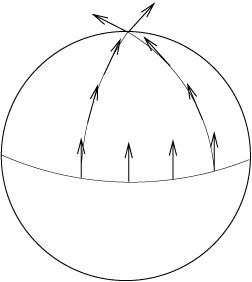
\includegraphics[scale=0.5]{image/sc}
			\caption{In a sphere start with a vector on the equator, pointing along a line of constant longitude. Parallelly transport it up to the north pole along a line along longitude in the obvious way. Then take the original vector, parallel transport it along the equator by an angle $ \theta$, and then move it up to the north pole as before. It is clear that the vector, parallel transported along two paths, arrived at the same destination with two different values (rotated by $ \theta$).}
		\end{figure}

		To formulate these notions one has to define what is meant by \emph{parallel transport}.
		\begin{definition} 
			A vector field $X$ on $M$ is said to be parallely transported along a smooth curve $\gamma : \mathbb{R} \rightarrow M$ if $\nabla_{v_\gamma}X = 0$.
		\end{definition}
		\begin{definition}
			A curve $\gamma : \mathbb{R} \rightarrow M$ is called autoparallely transported if $\nabla_{v_\gamma}v_\gamma = 0$.
		\end{definition}
		\begin{remark}
			$v_\gamma$ is not exactly a vector field, it is only defined on the curve $\gamma$. So to make sense of the definition one has to analytically continue $v_\gamma$ throughout $M$ and then apply the above definition. However the continuation might not be unique. Fortunately one can show that value of the vectors outside the curve is irrelevent for the above definition hence the definition makes sense.
		\end{remark}
		Now lets look how the equation looks in a chart $(U,x)$.
		\begin{equation*}
			\begin{split}
				\nabla_{v_\gamma}v_\gamma &= \nabla_{\dot{\gamma}^{m}\tfrac{\partial}{\partial x^m}}\dot{\gamma}^{n}\tfrac{\partial}{\partial x^n}
				= \dot{\gamma}^m \tfrac{\partial \dot{\gamma}^{n}}{\partial x^m}\tfrac{\partial}{\partial x^n} + \dot{\gamma}^{m}\dot{\gamma}^{n}\Gamma_{mn}^{q}\tfrac{\partial}{\partial x^q}
				=\ddot{\gamma}^{q}\tfrac{\partial}{\partial x^q} + \dot{\gamma}^{m}\dot{\gamma}^{n}\Gamma_{mn}^{q}\tfrac{\partial}{\partial x^q}
			\end{split}
		\end{equation*}
		hence we get for an autoparallely transported curve
		\begin{equation*}
			\ddot{\gamma}^{q} + \Gamma_{mn}^{q}\dot{\gamma}^{m}\dot{\gamma}^{n} = 0
		\end{equation*}
		The equation is famously known as \emph{geodesic equation}. A particle without any external field in a manifold will follow the path described by this equation. \\ 
		For euclidean space $U = \mathbb{R}^2$ $x = id_{\mathbb{R}^2}$ and $\Gamma_{mn}^{q} = 0$. Then the geodesic equation becomes 
		\begin{equation*}
			\ddot{\gamma}^q = 0 \implies \gamma^q = a^q\lambda + b^q
		\end{equation*}
		which is exactly the equation of straight line.

	\section{Torsion}
		\begin{definition}
			The torsion of a connection $\nabla$ is the $(1,2)$-tensor field
			\begin{equation*}
				T(\omega,X,Y) := \omega\left(\nabla_{X}Y - \nabla_YX - [X,Y]\right)
			\end{equation*}
			where $[X,Y]$ is a vector field defined such a way that $[X,Y]f := X(Yf) - Y(Xf)$.
		\end{definition}
		In a chart,
		\begin{equation*}
			\begin{split}
				T_{jk}^{i} :&= T\left(dx^i,\tfrac{\partial}{\partial x^j},\tfrac{\partial}{\partial x^k}\right) \\
				&= dx^i\left(\nabla_{\tfrac{\partial}{\partial x^j}}\tfrac{\partial}{\partial x^k} - \nabla_{\tfrac{\partial}{\partial x^k}}\tfrac{\partial}{\partial x^j} - \left[\tfrac{\partial}{\partial x^j},\tfrac{\partial}{\partial x^k}\right]\right) \\
				&= \Gamma_{kj}^{i} - \Gamma_{jk}^{i} - 0
			\end{split}
		\end{equation*}
		The last term vanishes as partial derivatives commute with each other. 
		\begin{definition}
			A smooth manifold $M$ with a connection is called torsion-free if $T = 0$.
		\end{definition}
		In terms of Christoffel symbols this translates to the fact that $\Gamma_{jk}^{i}$ is symmetric under two lower indices i.e. $\Gamma_{kj}^{i} = \Gamma_{jk}^{i}$. The assumption that a manifold is torsion-free is always taken in General Relativity. Geometrical significance of this assumption is not clearly understood.
	\section{Curvature}
		\begin{definition}
			Riemann curvature of a connection is the $(1,3)$-tensor field
			\begin{equation*}
				R(\omega,Z,X,Y) := \omega\left(\nabla_X\nabla_YZ - \nabla_Y\nabla_XZ - \nabla_{[X,Y]}Z\right)
			\end{equation*}
		\end{definition}
		To get the idea why this measures the curvature of space note that the covariant derivative of a tensor in a certain direction measures how much the tensor changes relative to what it would have been if it had been parallel transported (since the covariant derivative of a tensor in a direction along which it is parallel transported is zero). The commutator of two covariant derivatives, then, measures the difference between parallel transporting the tensor first one way and then the other, versus the opposite ordering as shown by the picture below. 
		Components of Riemann tensor-field in a chart has the following form
		\begin{equation*}
			R^{a}_{bcd} = \partial_c\Gamma^{a}_{bd} - \partial_d\Gamma^{a}_{bc} +\Gamma^{e}_{bd}\Gamma^{a}_{ec} + \Gamma^{e}_{bc}\Gamma^{a}_{ed}
		\end{equation*}
		where $\partial_c := \tfrac{\partial}{\partial x^c}$. From the above equation it can be easily seen that $R$ is antisymmetric in its last two entry.
		And one can also show by computation that
		\begin{equation*}
			\left[\nabla_{\mu},\nabla_{\nu}\right]X^{\rho} = R_{\sigma \mu \nu}^{\rho}X^{\sigma} - T_{\mu \nu}^{\lambda}\nabla_{\lambda}X^{\rho}
		\end{equation*}
		where $\nabla_{\mu} = \nabla_{\tfrac{\partial}{\partial x^\mu}}$.
		\begin{figure}[H]
			\centering
			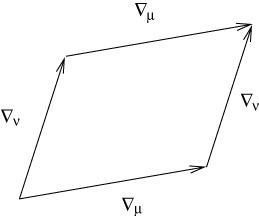
\includegraphics[scale=0.5]{image/cr}
			\caption{Geometric interpretation of Riemann tensor}
		\end{figure}
		Riemann tensor is extremely important in general relativity. Here is some properties of the components $R^{a}_{bcd}$.
		\begin{equation*}
			R^{a}_{bcd}+R^{a}_{cdb}+R^{a}_{dbc} = 0
		\end{equation*}
		\begin{equation}\label{Bianchi}
			\partial_eR^{a}_{bcd}+\partial_dR^{a}_{bec}+\partial_cR^{a}_{bde} = 0
		\end{equation}
		where the last identity is termed as Bianchi identity.\\ Riemann tensor is the key to measure curvature in a differentiable manifold. It essentially captures the geometry of the manifold. Not to say, it plays a central role in General relativity, though in GR one only needs a restricted knowledge of the Riemann tensor, namely its contraction, the  Ricci tensor. Contraction of 1st and 3rd indices of Riemann tensor produces the Ricci tensor $R_{bd} := R_{bad}^{a}$. We are using same notation for both Riemann tensor as well as Ricci tensor but this should not confuse the reader as the number of indices are different. Note that Ricci tensor is symmetric in its two indices i.e. $R_{ab}=R_{ba}$. Also one can define a scalar called Ricci scalar by contracting Ricci tensor with the metric tensor $R=g^{ab}R_{ab}$. This scalar also captures the curvature of space but not quite as accurate as Riemann tensor. But neverthless it is very important in GR. There is one more important tensor left to be defined. Einstien tensor $G_{ab}$ which is defined to be component-wise as
		\begin{equation*}
			G_{ab} = R_{ab}-\tfrac{1}{2}g_{ab}R
		\end{equation*}  This tensor has one very interesting property that it's divergence is zero i.e. $\nabla_{\tfrac{\partial}{\partial x^b}}G_{ab} = 0$. This can be proven using Bianchi identity. This fact will be used later.\\
		Above paragraph consists of various example of tensors and scalar which measure the curvature at a point in a differential manifold. Those are enough to talk about geometry of curved space as far as General Relativity is concerned. Now that we have developed how to talk about the curvature of space (spacetime) next order of business will be to understand what changes the curvature and a self-consisting equation relating the two to determine the dynamics of a particle in spacetime.
	\section{Energy Momentum Tensor}
		The most important tensor in physics, especially in astrophysics, is the energy-momentum tensor. As the name suggests, this tensor keeps track of energy and momentum densities in space-time. Historically, this tensor is written as $T$. One can expect this tensor to be dependent on the system of interest. In mechanics we encode all the information of the system in a single scalar called Lagrangian $\mathcal{L}$. Components of energy momentum tensor $T_{ab}$ can be derived from the Lagrangian as follows:
		\begin{equation*}
			T^{ab} = \tfrac{\partial \mathcal{L}}{\partial (\partial _a \phi)}\partial^b \phi - g^{ab}\mathcal{L}
		\end{equation*}
		Here are few examples of energy-momentum tensors
		\begin{itemize}
			\item \textit{Isolated Particle}: $T^{ab}(\textbf{x},t) = \dfrac{mv^a(t)v^b(t)}{\sqrt{1-(v/c)^2}}\delta(\textbf{x}-\textbf{x}_p(t))$ where $\textbf{x}_p(t)$ is the trajectory of the particle.
			\item \textit{Perfect fluid in equlibrium}: $T^{ab} = \left(\rho + \tfrac{p}{c^2}\right)u^au^b + pg^{ab}$ where $\rho$ and $p$ are respectively the density and pressure of the fluid.
			\item \textit{Electromagnetic Energy-momentum tensor}: $T^{ab} = \frac{1}{\mu_0}\left(F^{ac}g_{cd}F^{bd} - \frac{1}{4}g^{ab}F_{cd}F^{cd}\right)$ where $F^{ab}$ is the electromagnetic field tensor.
		\end{itemize}
		The components of energy-momentum tensor can be interpreted as follows:\emph{ $T^{ab}$ is the flux of $a^{th}$ component of the momentum vector across a surface with constant $x^{b}$ co-ordinate}. In relativity, momentum refers to the four-momentum. In this case time-time component is the density of relativistic mass i.e. the energy density divided by $c^2$. Flux of relativistic mass across $x^i$ surface is represented in the component $T^{0i}$. $T^{ii}$ (not summed) represents the normal stress i.e. pressure whereas $T^{ik}$ represent shear stress where $i,k$ take values 1,2,3.
		\\ Energy momentum tensor in General relativity is symmetric in its components i.e. $T^{ab} = T^{ba}$. Also, from energy and momentum conservation we have the following relation:
		\begin{equation*}
			\nabla_{\tfrac{\partial}{\partial x^b}}T^{ab} = 0
		\end{equation*}
		or equivalently $\nabla_{\tfrac{\partial}{\partial x^b}}T_{ab} = 0$.
	\section{Einstein Equation}
		We have developed how to describe curvature in space(space-time) and defined energy momentum tensor which represents the mass distribution, the source of curvature. Einstein equation relates these two quantities to get a field equation. Lets try to get to the equation by some informal reasoning and analogy and of-course,a little bit of hand-waving. \\ 
		We seek an equation much like Maxwell equation in electromagnetism, motivated from Newtonian Gravity, namely Poisson equation
		\begin{equation*}
			\nabla^2\Phi = 4\pi G\rho
		\end{equation*}
		The right hand side represents the mass density $\rho$ which we are tempted to replace with the energy-momentum tensor. Whereas the left hand side Laplacian of gravitational potential should be replaced by curvature of space as argued by Einstein using \emph{Equivalence Principle}. Curvature is given by Riemann tensor, Ricci tensor and Ricci scalar. Which one should we use? Also the metric tensor $g_{ab}$ encodes local curvature. Riemann tensor option can be ruled out as the right hand side contains only two indices. So some combination of Ricci tensor, Ricci scalar and metric tensor is the most general choice of the left hand side. But note that by energy conservation ,we have that the divergence of the right hand side has to be zero. So, for consistency we need divergence of the left hand side to vanish. Only one combination of $R_{ab}$, $R$ and $g_{ab}$ is divergenceless, which has been introduced earlier, the Einstein Tensor $G_{ab}$. Hence the final equation should look like
		\begin{equation*}
			G_{ab}  = \kappa T_{ab}
		\end{equation*} 
		or in full glory 
		\begin{equation*}
			R_{ab} - \tfrac{1}{2}Rg_{ab}  = \kappa T_{ab}
		\end{equation*} 
		where $\kappa = \tfrac{8\pi G}{c^2}$ is a constant which can be fixed by taking limits to Newtonian gravity. 
	
	\section*{Reference}
		\begin{enumerate}
			\item SPACETIME AND GEOMETRY: An introduction to General Relativity; Carroll, Sean ISBN 0-8053-8732-3
			\item MANIFOLD THEORY: An introduction for mathematical physicists; Martin, Daniel ISBN 0-13-543877-2
			\item  Lecture notes on General Relativity S. Carroll: \href{https://ned.ipac.caltech.edu/level5/March01/Carroll3/Carroll3.html}{https://ned.ipac.caltech.edu/level5/March01/Carroll3/Carroll3.html}
			\item \href{https://www.youtube.com/playlist?list=PLPH7f_7ZlzxTi6kS4vCmv4ZKm9u8g5yic}{Lectures on Geometrical Anatomy of Theoretical Physics} by Fredric P. Schuller given at Friedrich-Alexander-Universität Erlangen-Nürnberg.
			\item \href{https://www.youtube.com/watch?v=7G4SqIboeig&list=PLMsYJgjgZE8hh6d6ia2dP1NI0BKNRXbiw}{Lectures from the WE-Heraeus International Winter School on Gravity and Light
			} given by Fredric P. Schuller in 2015.
		\end{enumerate}

\end{document}
